\subsection{Aladin, Impact, and Calder kinetic codes}
\label{sec:AladinImpactCaldercodes}

\begin{figure}[tbh]
  \begin{center}
    \begin{tabular}{c}
      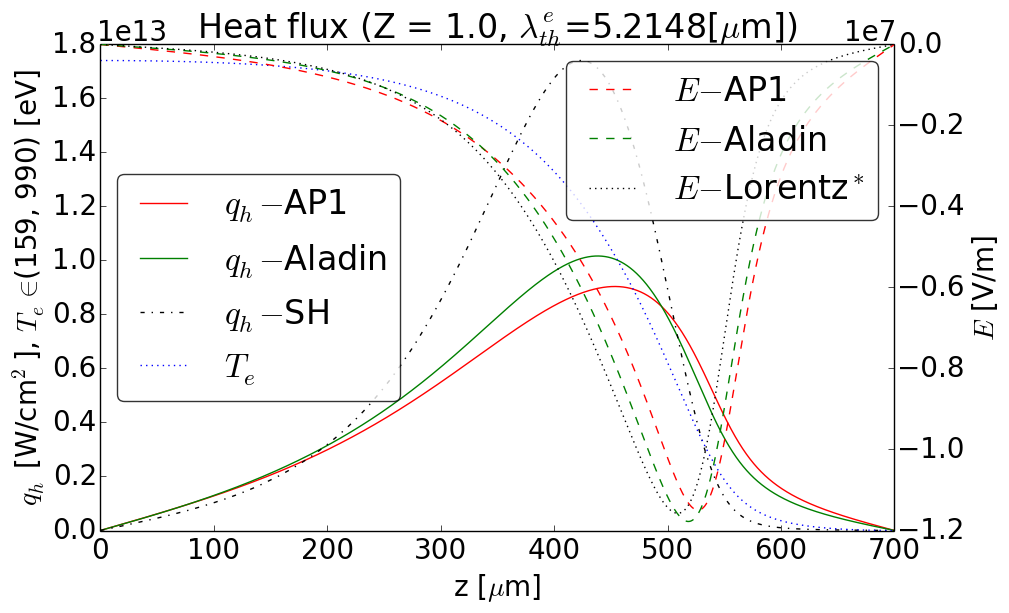
\includegraphics[width=\figscale\textwidth]{../VFPdata/C7_Aladin_case5_heatflux.png} \\
      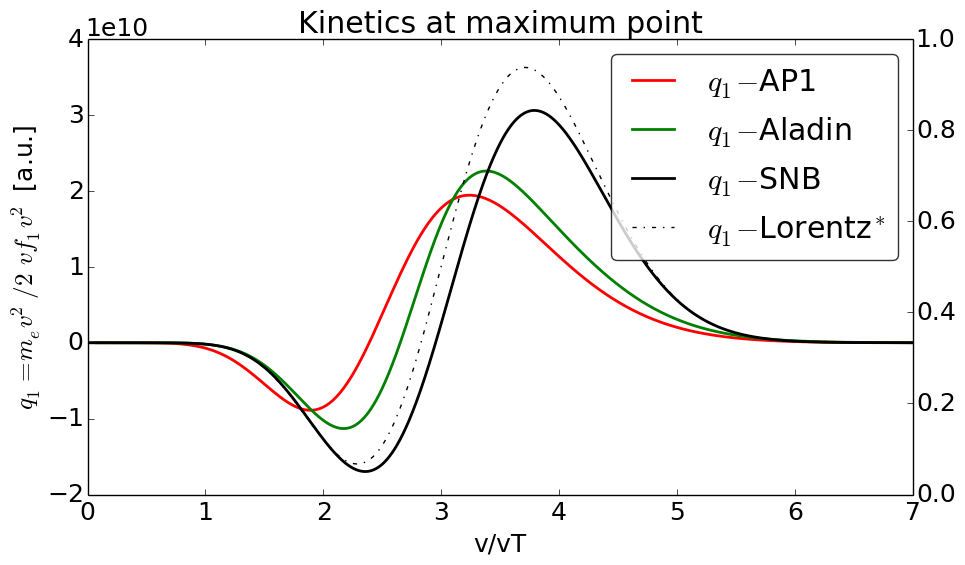
\includegraphics[width=\figscale\textwidth]{../VFPdata/C7_Aladin_case5_kinetics.png}
    \end{tabular}
  \caption{  
  Snapshot 20 ps. Left: correct steady solution of heat flux. 
  Right: Aladins results are correct. Velocity limit 4.4 $\vth$..
  }
  \label{fig:C7_Aladin_case5}
  \end{center} 
\end{figure}

%\begin{figure}[tbh]
%  \begin{center}
%    \begin{tabular}{c}
%      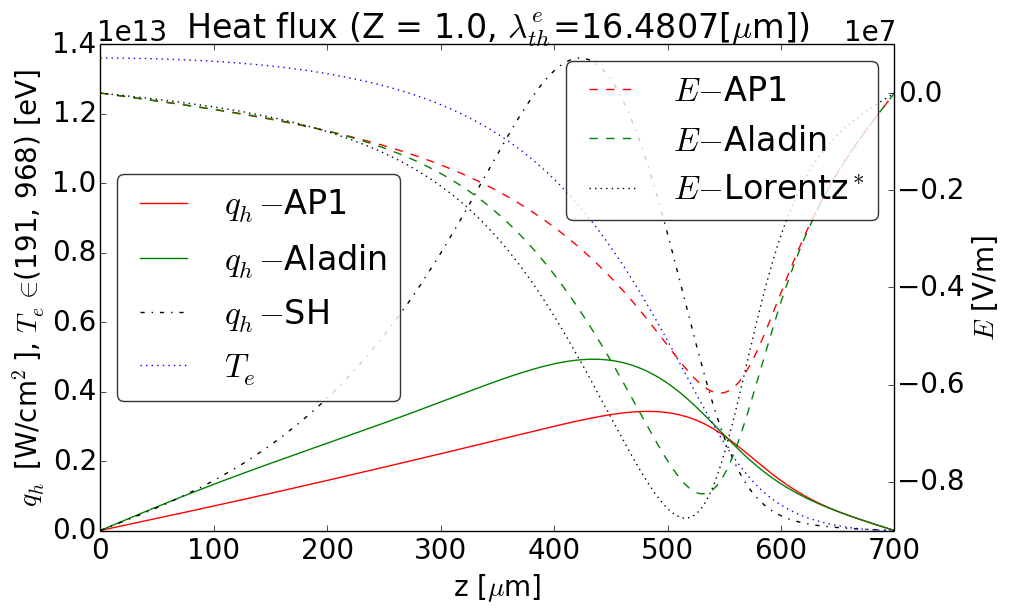
\includegraphics[width=\figscale\textwidth]{../VFPdata/C7_Aladin_case6_heatflux.png} \\
%      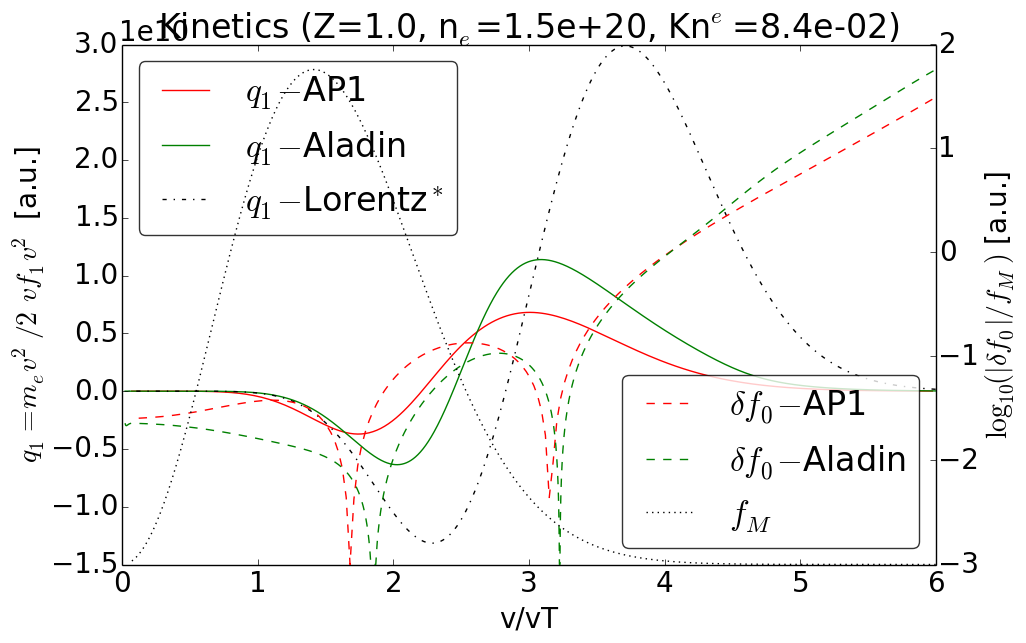
\includegraphics[width=\figscale\textwidth]{../VFPdata/C7_Aladin_case6_kinetics.png}
%    \end{tabular}
%  \caption{  
%  Snapshot 20 ps. Left: correct steady solution of heat flux. 
%  Right: Aladins results are correct. Velocity limit 3.2 $\vth$..
%  }
%  \label{fig:C7_Aladin_case6}  
%  \end{center} 
%\end{figure}

\begin{figure}[tbh]
  \begin{center}
    \begin{tabular}{c}
      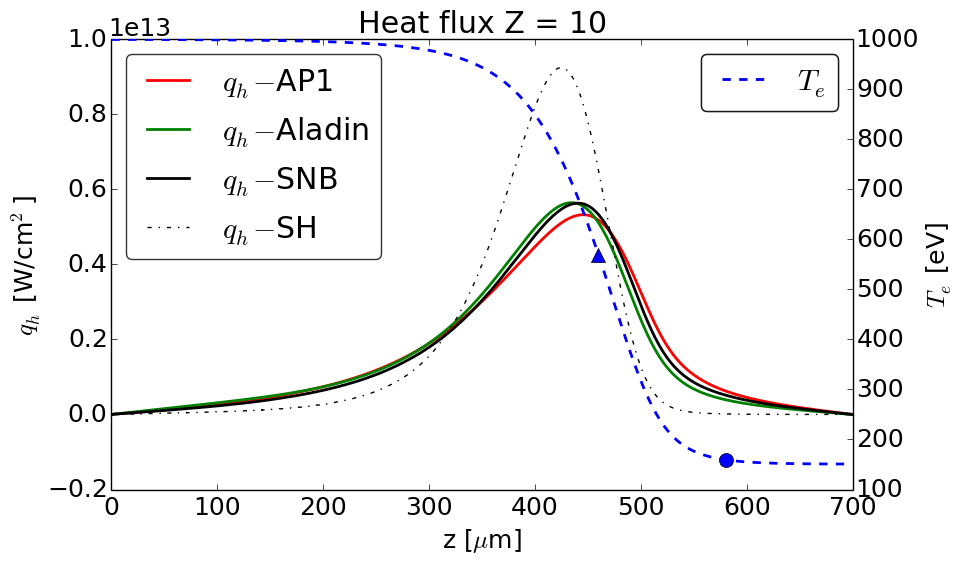
\includegraphics[width=\figscale\textwidth]{../VFPdata/C7_Aladin_case3_heatflux.png} \\
      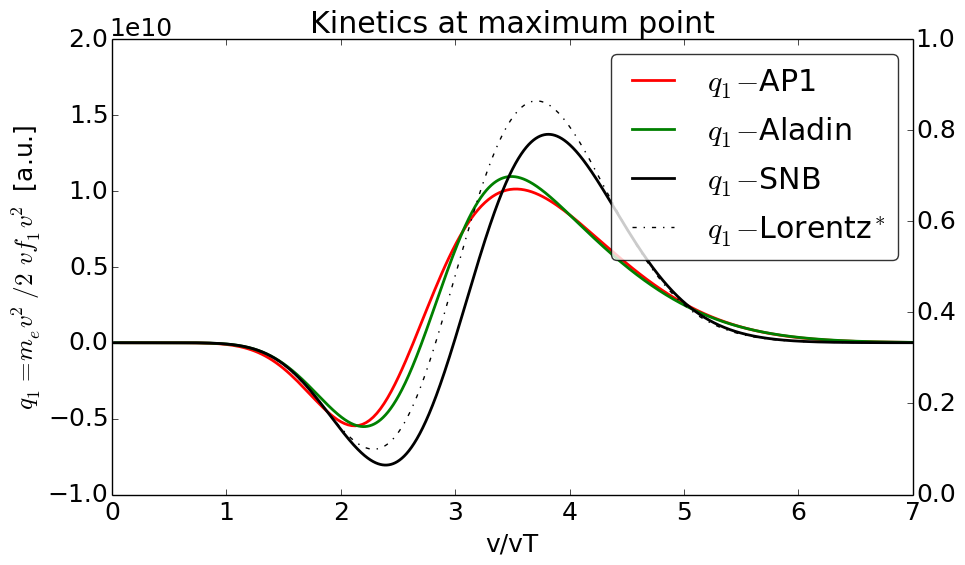
\includegraphics[width=\figscale\textwidth]{../VFPdata/C7_Aladin_case3_kinetics.png}
    \end{tabular}
  \caption{  
  Snapshot 12 ps. Left: correct steady solution of heat flux. 
  Right: correct comparison to kinetic profiles at point 442 $\mu$m by Aladin. 
  Velocity limit 3.4 $\vth$.
  }
  \label{fig:C7_Aladin_case3}
  \end{center} 
\end{figure}

\begin{itemize}
  \item Brief description of the Aladin code \figref{fig:C7_Aladin_case5}, \figref{fig:C7_Aladin_case3}. %\figref{fig:C7_Aladin_case6}
\end{itemize}

\begin{figure}[tbh]
  \begin{center}
    \begin{tabular}{c}
      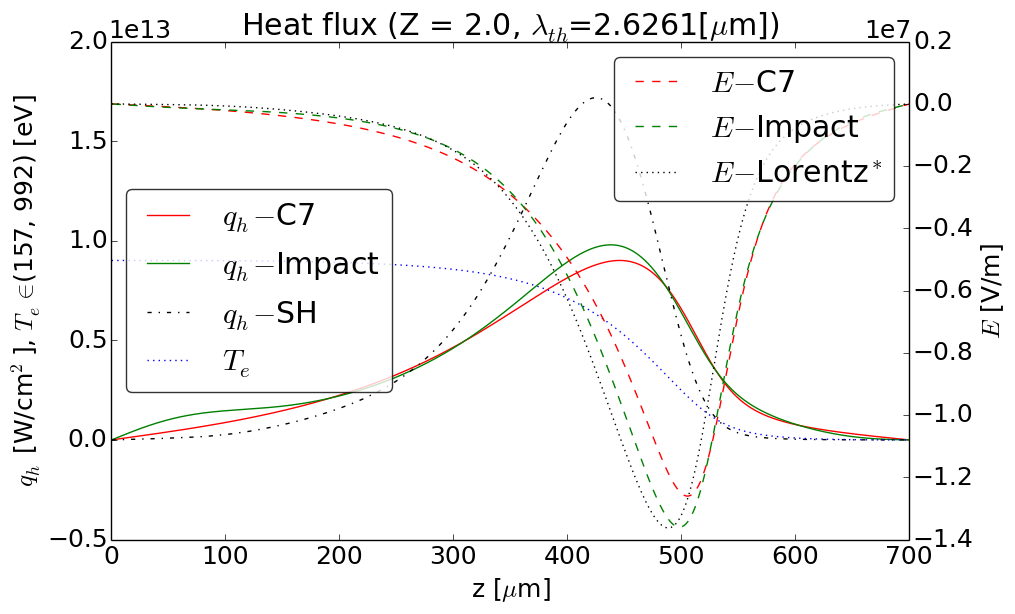
\includegraphics[width=\figscale\textwidth]{../VFPdata/C7_Impact_case3_heatflux.png} \\
      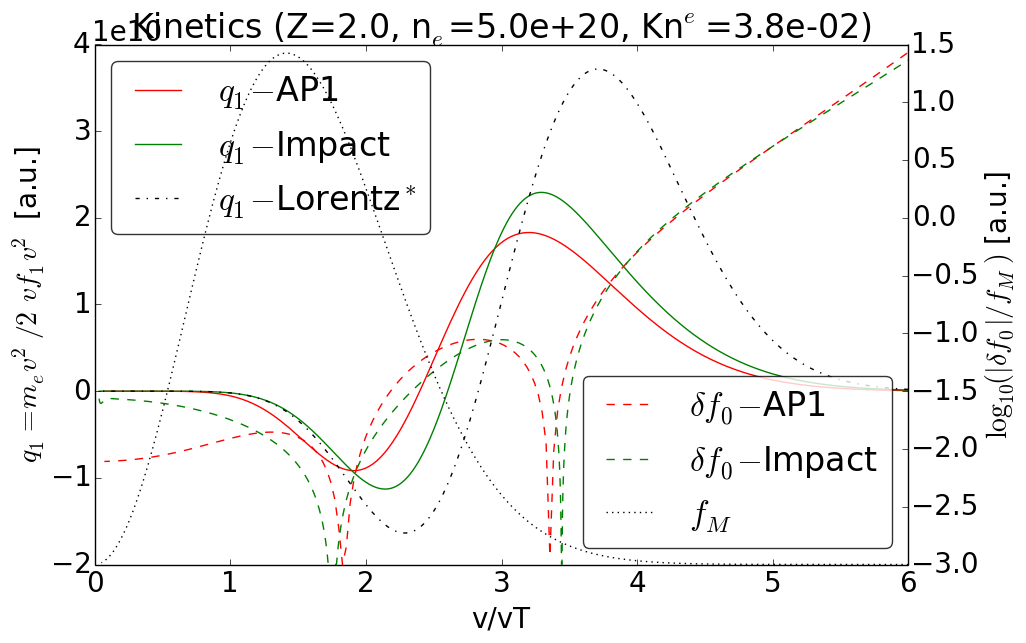
\includegraphics[width=\figscale\textwidth]{../VFPdata/C7_Impact_case3_kinetics.png}
    \end{tabular}
  \caption{  
  Snapshot 12 ps. Left: correct steady solution of heat flux. 
  Right: correct comparison to kinetic profiles at point 437 $\mu$m by Impact.
  Velocity limit 4.0 $\vth$.
  }
  \label{fig:C7_Impact_case3}
  \end{center} 
\end{figure}

\begin{itemize}
  \item Brief description of the Impact code \figref{fig:C7_Impact_case3}.
\end{itemize}

\begin{figure}[tbh]
  \begin{center}
    \begin{tabular}{c}
      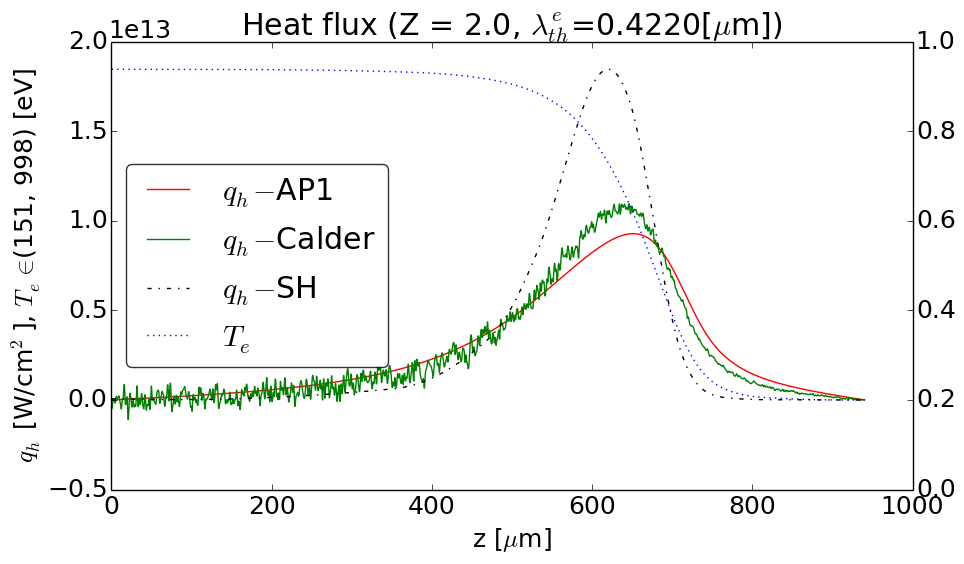
\includegraphics[width=\figscale\textwidth]{../VFPdata/C7_Calder_case1_heatflux.png} 
	  %\\ 
      %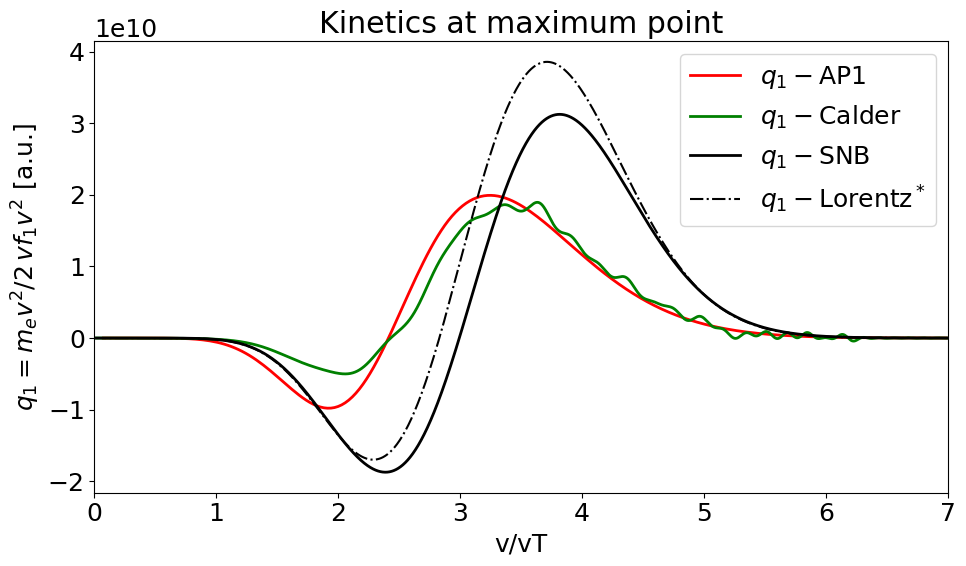
\includegraphics[width=\figscale\textwidth]{../VFPdata/C7_Calder_case1_kinetics.png}
    \end{tabular}
  \caption{  
  Snapshot 11 ps. Left: correct steady solution of heat flux. 
  Right: Kinetic profiles at point of maximum flux by AP1. 
  Kinetics profiles by CALDER should be added. Velocity limit 3.8 $\vth$.
  }
  \label{fig:C7_Calder_case1}
  \end{center} 
\end{figure}

\begin{itemize}
  \item Brief description of the Calder code \figref{fig:C7_Calder_case1}.
\end{itemize}
